
\chapter{Modelagem FrameWeb}
\label{sec-frameweb}
\vspace{-1cm}

\emph{\imprimirtitulo} é um sistema Web cuja arquitetura utiliza \textit{frameworks} comuns no desenvolvimento para esta plataforma. Desta forma, o sistema pode ser modelado utilizando a abordagem FrameWeb~\cite{souza-celebratingfalbo20}.

A Tabela~\ref{tabela-frameworks} indica os \textit{frameworks} presentes na arquitetura do sistema que se encaixam em cada uma das categorias de \textit{frameworks} que FrameWeb dá suporte. Em seguida, os modelos FrameWeb são apresentados para cada camada da arquitetura.

%\vitor{Substituir os valores da segunda coluna da Tabela~\ref{tabela-frameworks} pelos \textit{frameworks} utilizados no seu projeto. Remover o \hl{fundo amarelo}.}


\begin{footnotesize}
	\begin{longtable}{|c|c|}
		\caption{\textit{Frameworks} da arquitetura do sistema separados por categoria.}
		\label{tabela-frameworks}\\\hline
		
		\rowcolor{lightgray}
		\textbf{Categoria de \textit{Framework}} & \textbf{\textit{Framework} Utilizado} \\\hline 
		\endfirsthead
		\hline
		\rowcolor{lightgray}
		\textbf{Categoria de \textit{Framework}} & \textbf{\textit{Framework} Utilizado} \\\hline 
		\endhead

		Controlador Frontal & Spring MVC \\\hline

		Injeção de Dependências & Spring Framework \\\hline

		Mapeamento Objeto/Relacional & Spring Data JPA \\\hline

		Segurança & Spring Security \\\hline
	\end{longtable}
\end{footnotesize}




\section{Camada de Negócio}
\label{sec-frameweb-negocio}

%\vitor{Apresentar os modelos de entidades e de aplicação do FrameWeb.}

A figura~\ref{domain} mostra o projeto da Camada de Negócio (pacote \textsf{domain}) do sistema.

\begin{figure}[h]
	\centering
	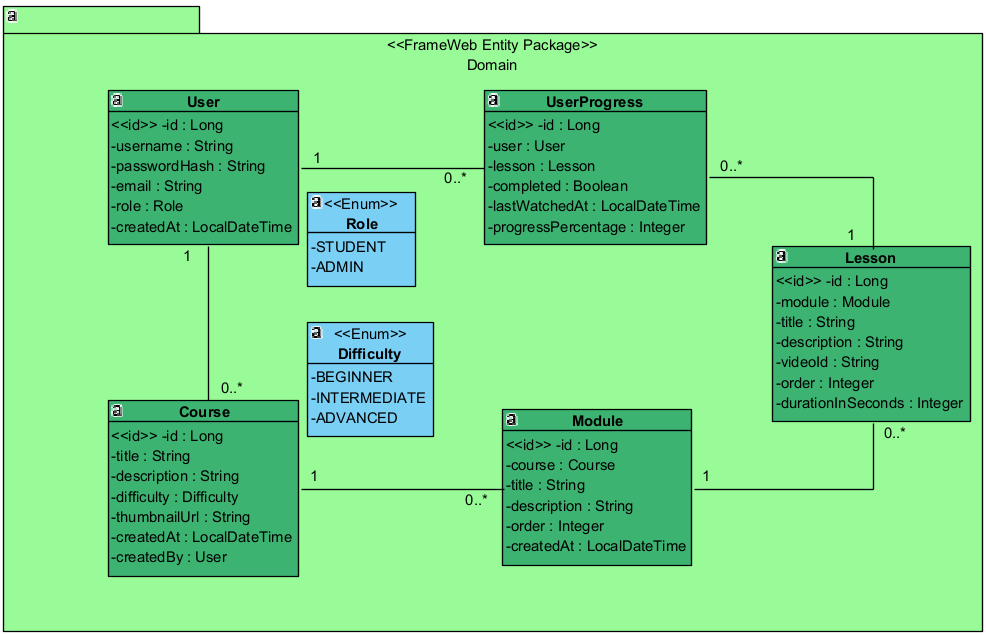
\includegraphics[width=0.8\textwidth]{figuras/domain.png}
	\caption{Projeto da Camada de Negócio (\textsf{domain})}
	\label{domain}
\end{figure}

Dentro do pacote \textsf{domain}, existem as entidades em verde escuro que são usadas como base das regras de negócio e da persistência de dados; enquanto as classes em azul claro, são tipos enumerados que representam classificações de usuário dentro do sistema (\textsf{Role}) e identificação da dificuldade de um curso (\textsf{Difficulty}).

\section{Camada de Acesso a Dados}
\label{sec-frameweb-dados}

%\vitor{Apresentar os modelos de persistência do FrameWeb.}

A figura~\ref{persistence} mostra o projeto da Camada de Acesso a Dados (pacote \textsf{persistence}) do sistema.

\begin{figure}[h]
	\centering
	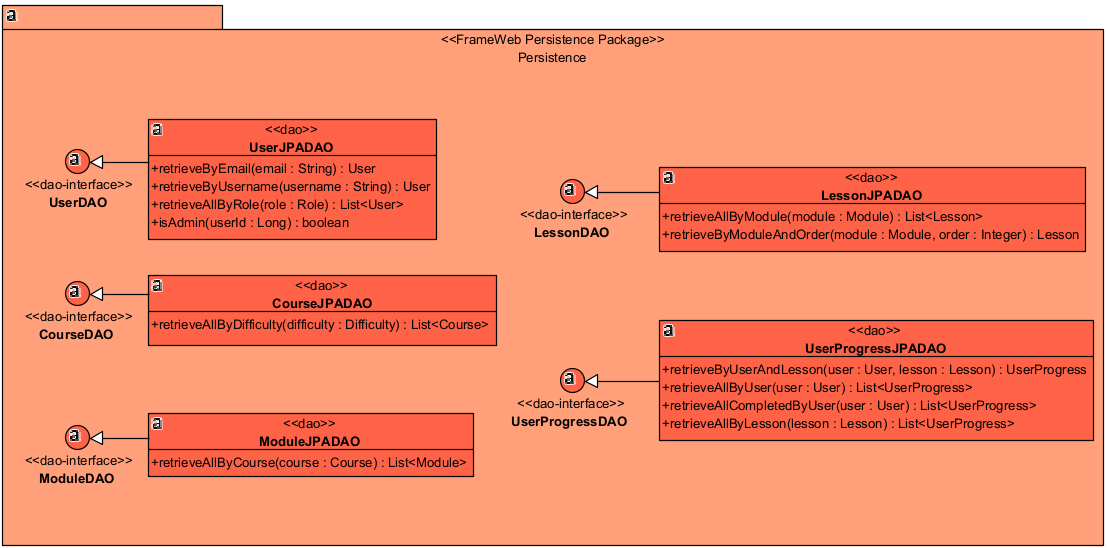
\includegraphics[width=0.8\textwidth]{figuras/persistence.png}
	\caption{Projeto de Acesso a Dados (\textsf{persistence})}
	\label{persistence}
\end{figure}

Nessa camada, como estará sendo utilizado o \textsf{Spring Data JPA}, por padrão ele já tem as buscas como create, read, update e delete (CRUD) das entidades básicas. Então, dentro de cada JPADAO do pacote \textsf{persistence} terão seus métodos personalizados que variam de acordo com a necessidade de acesso a dados do backend para aplicar suas regras de negócio que vão ser passadas ao \textsf{frontend}.

Enquanto o \textsf{Spring Data JPA}, há os métodos personalizados que fazem:

\begin{itemize}
	\item \textbf{UserJPADAO}: autenticação, recuperação de senha, validação de cadastro, cadastro/validação de nomes únicos, listar todos os alunos ou administradores e garantir que o usuário está acessando a área administrativa.
	
	\item \textbf{CourseJPADAO}: visualizar detalhes de um curso, vincular módulos a um curso, filtrar cursos por dificuldade.
	
	\item \textbf{ModuleJPADAO}: listar todos os módulos de um curso quando o aluno entra no curso.
	
	\item \textbf{LessonJPADAO}: listar as aulas dentro de um módulo, buscar uma aula específica em uma ordem (ex: próxima aula).
	
	\item \textbf{UserProgressJPADAO}: verificar se o aluno já completou a lição, listar progresso completo do aluno (quais aulas ele já viu), exibir o número de lições concluídas e estatísticas da aula: quantos alunos viram aquela lição.
\end{itemize}

\section{Camada de Apresentação}
\label{sec-frameweb-apresentacao}

\vitor{Apresentar os modelos de navegação do FrameWeb.}

adpoaskdpoasjkdpoasjdpoasjkdpoasjdposajdopasjdpoasdpoasdopasdpoasjdposajdpoasjdopj
adpoaskdpoasjkdpoasjdpoasjkdpoasjdposajdopasjdpoasdpoasdopasdpoasjdposajdpoasjdopj
adpoaskdpoasjkdpoasjdpoasjkdpoasjdposajdopasjdpoasdpoasdopasdpoasjdposajdpoasjdopj
adpoaskdpoasjkdpoasjdpoasjkdpoasjdposajdopasjdpoasdpoasdopasdpoasjdposajdpoasjdopj
adpoaskdpoasjkdpoasjdpoasjkdpoasjdposajdopasjdpoasdpoasdopasdpoasjdposajdpoasjdopj
adpoaskdpoasjkdpoasjdpoasjkdpoasjdposajdopasjdpoasdpoasdopasdpoasjdposajdpoasjdopj
